%\documentclass[11pt,xcolor=gray,handout]{beamer}
\documentclass[hyperref={pdfpagelabels=false}]{beamer}
\let\Tiny=\tiny
\mode<presentation>{
\usetheme{Singapore}
%\usecolortheme{lily}
\usefonttheme{serif}
}
\usepackage{default}
\usepackage{verbatim}
%\usepackage{ucs}
\usepackage[utf8]{inputenc}
\usepackage{gb4e}
\usepackage[T1]{fontenc}
\usepackage{ tipa }
\usepackage{qtree}
\usepackage{synttree}
\usepackage{color}
\usepackage{tree-dvips}
\usepackage[absolute,overlay]{textpos}
%\usepackage{covington-beamer}
\usepackage{lmodern}
\usepackage{natbib}
\usepackage{graphicx}
%\usepackage{pdfpages}


%\usepackage{memoir}
%\usepackage{relsize}
%\newcommand{\subscript}[1]{\raisebox{-0.25em}{\smaller #1}}
%\logo{\includegraphics[height=0.5cm]{hilogo2.png}}
\setbeamertemplate{footline}[frame number] 
%gets rid of navigation symbols
\setbeamertemplate{navigation symbols}{}

\title{Optionality is Stable Variation is Competing Grammars}
\author{Joel C. Wallenberg and Josef Fruehwald\\Newcastle University, University of Pennsylvania}
\institute{}
%\date[]{March 18, 2013 \\ University of Oslo}

\begin{document}

\begin{frame}[plain]
\titlepage
\end{frame}


\section{Introduction}
\begin{frame}{Introduction}
	Variation in grammar is often described as falling into one of two categories.
	
	\begin{enumerate}
		\item Competing Grammars
		\begin{itemize}
			\item Leads to language change via the replacement of one grammatical process by another.
			\item Competition is parameterized in some fashion, as in competing flavors of the same functional head \citep{kroch1994}.
		\end{itemize}
		\item Optionality (within a grammar?)
		\begin{itemize}
			\item Diachronically stable variation between grammatical processes.
		\end{itemize}
	\end{enumerate}
	
\end{frame}

\begin{frame}{Introduction}
	We will argue that grammatical optionality is formally the same as competing grammars, with the following consequences:
	\begin{itemize}
		\item The difference between language change and stable variation/optionality must be explained by some mechanism outside of the grammar itself. 
%		\item The linguistic system (and therefore the variation) interacts with various dimensions of language use, which have their own characteristics. 
%the (in)stability of a competing grammars situation
		\item We argue that it depends on the mathematical character of some extragrammatical dimension with which the variation interacts.
			\begin{itemize} \item Partial specialization of variants along a continuous dimension. \end{itemize}
%		\item Optionality in grammar must also be parameterized. The implications of this point are greater for stable phonological variation.
	\end{itemize}

\end{frame}

\begin{frame}
\frametitle{Outline}
\tableofcontents
\end{frame}


\section{Blocking and Contrast}
%Maybe revise presentation
\subsection{How doublets resolve, and why.}
\begin{frame}
\frametitle{Blocking and Contrast}
\begin{block}{``Blocking Effect''}
	\begin{itemize}
		\item General cognitive pressure against two forms existing for one function (``doublet'') (e.g. morphosyntactic doublets as in \citealt{kroch1994}).
		\item[ ]\{\textsl{dived, dove}\} (dive-\textsc{pst})\\ \{\textsl{jimmies, sprinkles}\} (candy topping)
		%\item The possible historical outcomes of a doublet are replacement (one form left) or specialisation (forms diverge in function).
	\end{itemize}
\end{block}
\begin{block}{``Principle of Contrast''}
	\begin{itemize}
		\item A strategy that children use in acquiring language: assume that two forms have two meanings (or uses)\citep[][{ \it inter alia}]{clark1987, clark1990}.
		\item Children hypothesize that novel words also refer to novel objects \citep[as in][among many other replications of the effect]{markmanwachtel1988}.
	\end{itemize}
\end{block}
%\begin{itemize}
%	\item General cognitive pressure against two forms existing for one function (``doublet''). 
%	\item This is the ``blocking effect'', as described for morphosyntactic doublets in Kroch (1994).\nocite{kroch1994}
%	\item The possible historical outcomes of a doublet are replacement (one form left) or specialisation (forms diverge in function).
%	\item Crucially, they do not coexist forever, nor does one variant die randomly.
%	\item Part of the blocking effect is a language acquisition strategy, the ``Principle of Contrast'' (E. Clark 1987); \citep[cf. also][and references therein]{clark1990}. \nocite{clark1987}
%\end{itemize}
\end{frame}

\begin{frame}
\frametitle{Blocking and Contrast}
\begin{itemize}
	\item A doublet is two variants competing for finite resources, as in e.g. biological evolution.
		\begin{itemize} 
			\item Instead of competing for something like food, they are competing for use (time in the mouths/brains of speakers) 
			%\item Selection operates on the number of times a variant is \textbf{heard} (i.e. and processed) by an acquirer. 		
			\end{itemize}
	\item Either one variant has an advantage, and so replaces the other \citep[following a logistic function;][]{nowak2006}.
	\item Or neither variant has an advantage, in which case random walk behaviour ensues.
	\item But in linguistic doublets, random walk cannot persist indefinitely because of the acquisition pressure of the Principle of Contrast.
\end{itemize}
\end{frame}

\begin{frame}
\frametitle{Competing Grammars}
\begin{itemize}
	\item This entire interpretation is dependent on some notion of ``competing grammars'' \citep{kroch1989, kroch1994}
	\item[ ] \textbf{Competing Grammars, general form}: 2 variants are available to a speaker with overlapping functions (e.g. the same meaning), and can't both be used at the same time.
		\begin{itemize}
			\item E.g. two featural versions of the same syntactic head. 
			\item E.g. two different output mappings for the same phonological input.
			\item E.g. two different spell-outs of a morpheme.
		\end{itemize}
	\item Necessary for the description of \textbf{any} linguistic change in a categorical dimension.
		\begin{itemize} 
			\item E.g. word-order parameters \citep{pintzuk1991, santorini1992}; a phonological rule like German final stop devoicing \citep{fruehwaldgresswallenberg}. 
			\item In any such case, a speaker in the middle of the change in progress (code-)switches between categorical variants.
		\end{itemize} 
\end{itemize}
\end{frame}


\begin{frame}{Blocking and Contrast}
	The possible historical outcomes of doublets (Competing Grammars) driven by the Blocking Effect and the Principle of Contrast are:
	\begin{itemize} 
		\item Replacement of one by the other.
		\item Specialization of the two forms to different functions or meaning.
	\end{itemize}

	\textbf{Proposal:} every case of categorical linguistic variation or optionality can be reduced to competing grammars, leading to one of these two outcomes.
	
	This simplifies the grammatical architecture necessary to account for both optionality and language change.
\end{frame}

%\subsection{The Principle of Contrast}
%\begin{frame}
%\frametitle{The Principle of Contrast}
%\begin{itemize}
%	\item A strategy that children use in acquiring language: assume that two forms have two meanings (or uses).
%		\begin{itemize} \item Synonyms should only be acquired as a last resort.\end{itemize}
%	\item Demonstrated many times, in experiments like \citet{markmanwachtel1988}.
%		\begin{enumerate}
%			\item 20 children
%			\item 6 pairs of one familiar item (banana, cow, cup, plate, saw, spoon) and one unfamiliar item (cherry pitter, odd shaped wicker container, lemon wedgepress, radish rosette maker, studfinder, tongs).
%			\item \textbf{Control}: ``Show me one''
%			\item \textbf{Test}: ``Show me the X'' (X = nonsense syllable)
%		\end{enumerate}
%	\item Control children pick the unfamiliar object at chance levels, but test children choose unfamiliar objects significantly higher than chance.
%\end{itemize}
%\end{frame}

%Talk more about Principle of Contrast

%
%\begin{frame}
%\frametitle{An Evolutionary Process}
%\begin{itemize}
%	\item Therefore, we propose that the Blocking Effect is reducible to Darwinian selection; it is just an evolutionary process.
%	\item A doublet resolves in replacement when one form has a selectional advantage.
%	\item A doublet resolves in specialisation when neither form has a selectional advantage (or a very small one).
%	\item Unlike biology, the Principle of Contrast is built into acquisition and prevents random walk.
%	\item In biology, a selectional advantage is a higher probability of reproduction.
%	\item In language change, a selectional advantage is a higher probability of a child hearing and acquiring a particular structure.
%\end{itemize}
%\end{frame}
%
%
\section{Competing Grammars}

%
%\begin{frame}
%\frametitle{Polar Qs and Competing Grammars}
%\begin{itemize}
%	\item The competing grammars situation (like all morphosyntactic doublets) is constrained to two possible outcomes \citep{kroch1994}, as the \textsl{whether/if} study shows:
%		\begin{itemize}
%			\item Replacement of one variant by the other.
%			\item Specialisation of each variant for a specific context over time.
%		\end{itemize}
%	\item \textbf{Proposal:} every case of syntactic variation or optionality can be reduced to competing grammars, in one of these two versions.
%	\item That is good, because competing syntactic heads is the only possible locus of variation/optionality in a BPS syntax.
%\end{itemize}
%\end{frame}
%
\subsection{Syntactic Optionality as Competing Grammars}
\begin{frame}
\frametitle{Example: English ``Topicalization''}
\begin{itemize}
	\item \citet{prince1985,prince1998, prince1999}: felicitous in two English discourse contexts, both of which require a certain type of contrast to appear on the fronted XP.
	
	\begin{exe}
\ex \label{princetop1} She's going to use three groups of mice.
One, she'll feed them mouse chow, just the regular stuff they make for
mice.
Another she'll feed them veggies.
And the third she'll feed junk food.\\

\ex \label{princetop2} She was here two years.
[checking transcript] Five semesters she was here.\\
\citep[][8,9]{prince1999} 

\end{exe}

	\item However, it is \textbf{never} obligatory.
\end{itemize}
\end{frame}
%
\begin{frame}
\frametitle{Example: English Topicalization}
\begin{itemize}
	\item As long as the accent pattern is kept constant, both orders are felicitous:
	
	\begin{exe}
\ex \label{princetop1} She's going to use three groups of mice.
One, she'll feed them mouse chow, just the regular stuff they make for
mice.
Another she'll feed them veggies.
And \textbf{the third} she'll feed \textbf{junk food}.\\

\ex \label{untop1} She's going to use three groups of mice.
One, she'll feed them mouse chow, just the regular stuff they make for
mice.
Another she'll feed them veggies.
And she'll feed \textbf{the third} \textbf{junk food}.\\

\end{exe}

\end{itemize}
\end{frame}
%
%\begin{frame}
%\frametitle{Example: English ``Topicalization''}
%\begin{itemize}
%	\item As long as the accent pattern is kept constant, both orders are felicitous:
%	\begin{exe}
%
%\ex \label{princetop2} She was here two years.
%[checking transcript] \textbf{Five semesters} she was here.\\
%
%\ex \label{untop2} She was here two years.
%[checking transcript] she was here \textbf{five semesters}.\\
%
%\end{exe}
%
%\end{itemize}
%\end{frame}
%
\begin{frame}
\frametitle{Topicalization in Minimalism}
\begin{itemize}
	\item Move is triggered by the feature content of some head.
	\item Given ``Merge...preempts Move'' \citep{chomsky2000}, a feature cannot encode optional movement.
	\item Therefore, optional movement must involve a choice (for the \textbf{Numeration}) between two variants of a functional head, out of an inventory of possible heads:
\end{itemize}
\vspace{2mm}

\Tree [.CP XP_i [.C' {C\\$[F]$} \qroof{...t_i...}.TP ] ] \Tree [.CP C \qroof{...XP...}.TP ]

\begin{itemize}
	\item This is the core case of morphosyntactic doublet (i.e. competing heads) described in \citet{kroch1994}.
\end{itemize}

\end{frame}

\subsection{A Minimalist Hypothesis for Variation/Optionality}
\begin{frame}
\frametitle{A Minimalist Hypothesis}
\begin{itemize}
	\item[ ] Given that: 
		\begin{itemize} 
		\item these mechanics are necessary to encode syntactic optionality in a Minimalist system,
		\item the same mechanics are necessary to describe a change in progress
		\end{itemize}
	\item[ ] Then, the system is simplest if no more machinery is added to deal with optionality/variation.
\end{itemize}

\end{frame}

\begin{frame}
\frametitle{A Minimalist Hypothesis}
\begin{itemize}
	\item \textbf{Prediction:} every case of syntactic optionality or variation is one of the following:
		\begin{enumerate}
			\item A replacement change in progress (outright competition going to completion).
			\item A specialisation change in progress (specialisation for different functions going to completion).
			\item \textbf{The only real case of diachronically stable variation/optionality:} variants have partially specialized along a continuous (or ordinal) dimension, e.g. style, prosodic weight. 
		\end{enumerate}
	\item If categorical variants specialize along a categorical dimension, complete specialisation should eventually result.
	\item If categorical variants specialize along a continuous or ordinal dimension, then complete specialisation can \textbf{never} result (but replacement can still be arrested).
\end{itemize}

\end{frame}

\subsection{Example: Embedded Polar Questions}

\begin{frame}
\frametitle{Example: Embedded Polar Questions}
A quantitative study of embedded \textsl{yes/no}-questions in English and Icelandic, comparing the use of \textsl{whether} vs. \textsl{if}, and \textsl{hvort} vs \textsl{ef} found specialisation in English, and replacement in Icelandic (Bailey, Wallenberg, \& van der Wurff 2012). \nocite{baileywallenbergwurff2012}\\
	\begin{exe}
		\ex John wondered whether Mary was coming to the party.
		\ex John wondered if Mary was coming to the party.
	\end{exe}
\end{frame}

\begin{frame}{Example: Embedded Polar Questions}
		In all stages of English and in historical Icelandic, a disjunction favors {\it whether}.
	\begin{block}{English}
		\begin{itemize}
		\item[ ]\textbf{Disjunction:}
		\begin{exe}
			\ex I wonder \{{\bf whether},if\} John or Bill is bringing coffee.
			\ex I wonder \{{\bf whether},if\} John is bringing tea or coffee.
			%\ex I wonder \{whether,if\} John is bringing tea or not.
		\end{exe}
		\item[ ]\textbf{Simple:}
		\begin{exe}
			\ex I wonder \{whether, {\bf if}\} Bill is bringing coffee.
		\end{exe}
		\end{itemize}
	
	\end{block}
\end{frame}

\begin{frame}{Example: Embedded Polar Questions}
%	\begin{block}{}
		\begin{itemize}
		\item[ ]\textbf{Disjunction:}
		\begin{exe}
			\ex \gll eftir því \textbf{hvort} maður vill heitt eða kalt\\
			according it-DAT whether man wants hot or cold\\
			\quad ``According to whether one wants hot or cold'' \\(\textsl{Sagan Öll}, date: 1985, from IcePaHC\nocite{icepahc09})
		\end{exe}
		\item[ ]\textbf{Simple, (older) Icelandic:}
		\begin{exe}
			\ex \gll vér vitum eigi, \textbf{hvort} vér tökum öndina\\
			We know not whether we take soul-the\\
			\ex \gll og spurðu, \textbf{ef} hann væri Kristur\\
			and asked if he were Christ\\
			(\textsl{Icelandic Homilies}, date: 1150, from IcePaHC)
		\end{exe}
		\end{itemize}		
%	\end{block}

\end{frame}






%\begin{frame}
%\frametitle{A Quantitative Study}
%\begin{itemize}
%	\item A quantitative study of embedded \textsl{yes/no}-questions in English and Icelandic, comparing the use of \textsl{whether} vs. \textsl{if}, and \textsl{hvort} vs \textsl{ef}.
%	\item \textbf{Result 1:} A strong predictor of \textsl{whether} vs. \textsl{if} in both languages is the presence/absence of a disjunction (i.e. \textsl{or, eða}) in the clause, with \textsl{whether} being favoured in the disjunction case more than in the simple case in both languages, across their whole histories.
%	\item This indicates a remarkably long-lasting ``persistence'' effect of the original reanalysis environment (inspired by \textsl{have} vs, \textsl{have got} study by Shawn Noble, reported in \citealt{kroch1989}, cf. also \citealt{labov1989}).
%	\item The effect supports our hypothesis about the reanalysis environment.
%\end{itemize}
%\end{frame}


%\begin{frame}
%\frametitle{A Quantitative Study}
%\begin{itemize}
%	\item \textbf{Result 2:} The \textsl{whether} structure completely replaces the \textsl{if} structure in the Icelandic case, but not in the English case.
%	\item If the two possible outcomes of a morphosyntactic doublet are replacement or specialisation \citep{kroch1994}, Icelandic shows the former and English shows the latter.
%	\item We propose that replacement must occur when there is some selectional advantage to one of the variants (in Darwinian terms, where reproduction = learning).
%	\item Specialisation must occur when there is no selectional advantage to one of the variants.
%	\item \textbf{Experimental Infrastructure:} accurate parsed diachronic corpora: \small{ YCOE \citep{ycoe}, PPCME2 \citep{ppcme2}, PPCEME \citep{ppceme}, PPCMBE \citep{ppcmbe}, and IcePaHC \citep{icepahc09}.}
%	
%\end{itemize}
%\end{frame}
%
%\begin{frame}
%\frametitle{English Examples}
%\begin{itemize}
%\item[ ]\textbf{Disjunction:}
%\begin{exe}
%	\ex I wonder \{whether,if\} John or Bill is bringing coffee.
%	\ex I wonder \{whether,if\} John is bringing tea or coffee.
%	\ex I wonder \{whether,if\} John is bringing tea or not.
%\end{exe}
%\item[ ]\textbf{Simple:}
%\begin{exe}
%	\ex I wonder \{whether,if\} Bill is bringing coffee.
%\end{exe}
%\end{itemize}
%\end{frame}
%
%\begin{frame}
%\frametitle{Icelandic Examples}
%\begin{itemize}
%\item[ ]\textbf{Disjunction:}
%\begin{exe}
%	\ex \gll eftir því \textbf{hvort} maður vill heitt eða kalt\\
%	according it-DAT whether man wants hot or cold\\
%	\quad ``According to whether one wants hot or cold'' \\(\textsl{Sagan Öll}, date: 1985, from IcePaHC, \citealt{icepahc09})
%\end{exe}
%\item[ ]\textbf{Simple, (older) Icelandic:}
%\begin{exe}
%	\ex \gll vér vitum eigi, \textbf{hvort} vér tökum öndina\\
%	We know not whether we take soul-the\\
%	\ex \gll og spurðu, \textbf{ef} hann væri Kristur\\
%	and asked if he were Christ\\
%	(\textsl{Icelandic Homilies}, date: 1150, from IcePaHC)
%\end{exe}
%\end{itemize}
%\end{frame}
%
%\begin{frame} 
% \frametitle{English \textsl{whether} vs. \textsl{if} Questions, N = 1929 clauses}
%
%\begin{center}
% 
% \begin{textblock*}{125mm}(0mm,14mm)
%\includegraphics[width=109mm,height=82mm,clip=true,trim=0mm 0mm 0mm 0mm]{whetherifEngSimple.pdf}
%\end{textblock*}
%%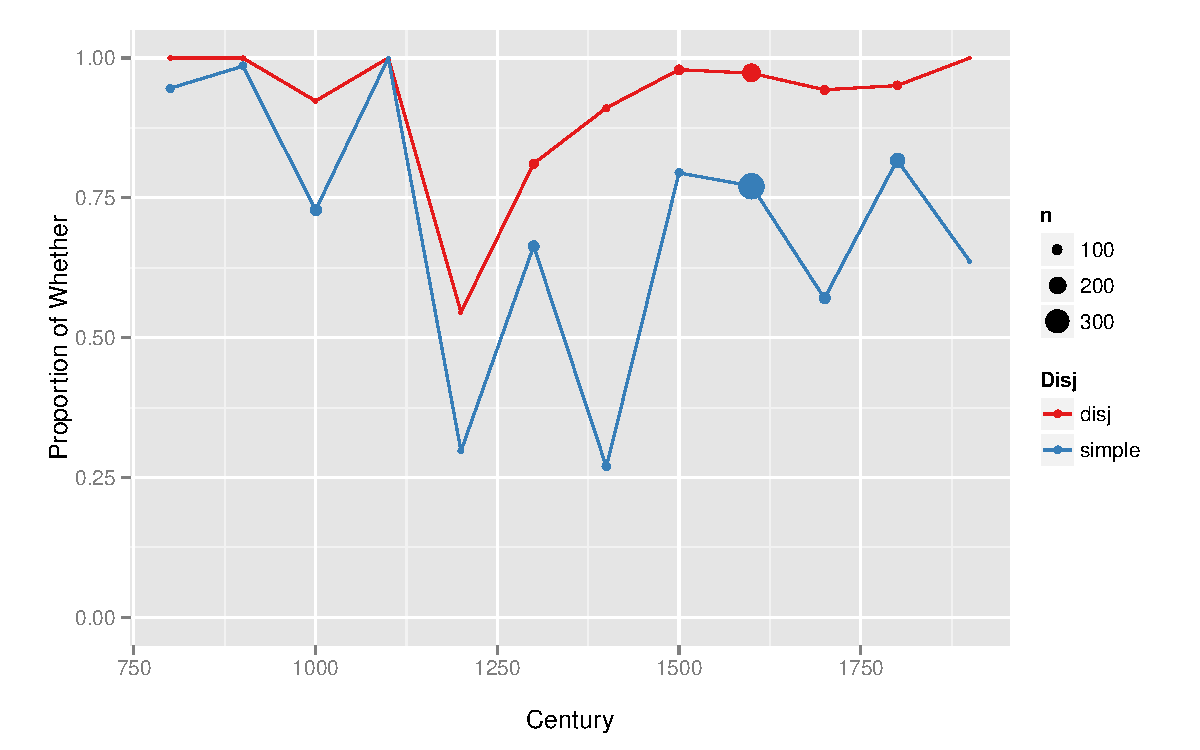
\includegraphics[scale = 0.5]{whetherifEng.pdf}
%\end{center}
%\end{frame}
%
%\begin{frame} 
% \frametitle{Icelandic \textsl{hvort} vs. \textsl{ef} Questions, N = 397 clauses}
%\begin{center}
% 
% \begin{textblock*}{125mm}(0mm,14mm)
%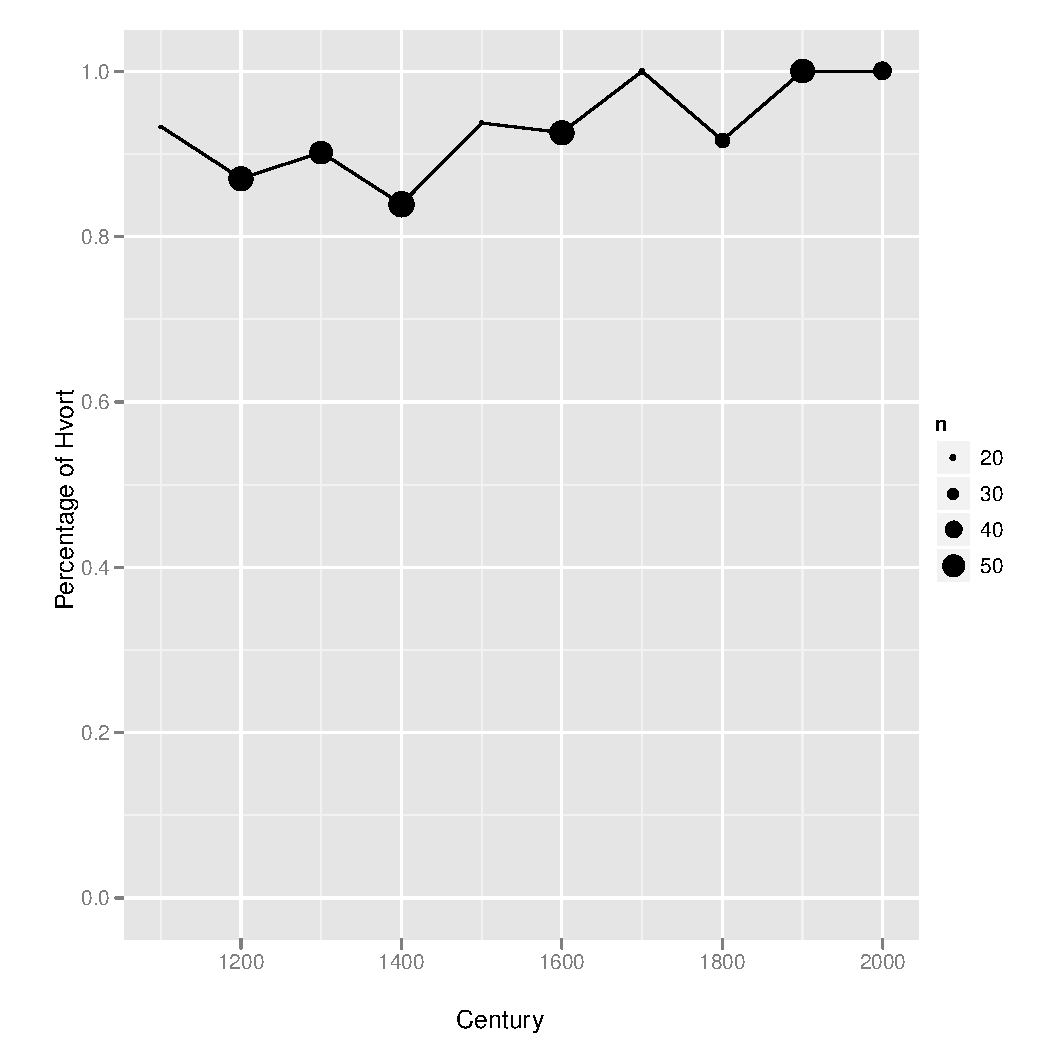
\includegraphics[width=109mm,height=80mm,clip=true,trim=0mm 0mm 0mm 0mm]{whetherifIceSimple.pdf}
%\end{textblock*}
%
%\end{center}
%\end{frame}
%
\begin{frame}{Specialisation in English (N = 1929 clauses)} 


\begin{center}
 \small{Parsed Corpora: YCOE, PPCME2, PPCEME, PPCMBE \nocite{ycoe,ppcme2,ppceme,ppcmbe}}
% \begin{textblock*}{125mm}(0mm,14mm)
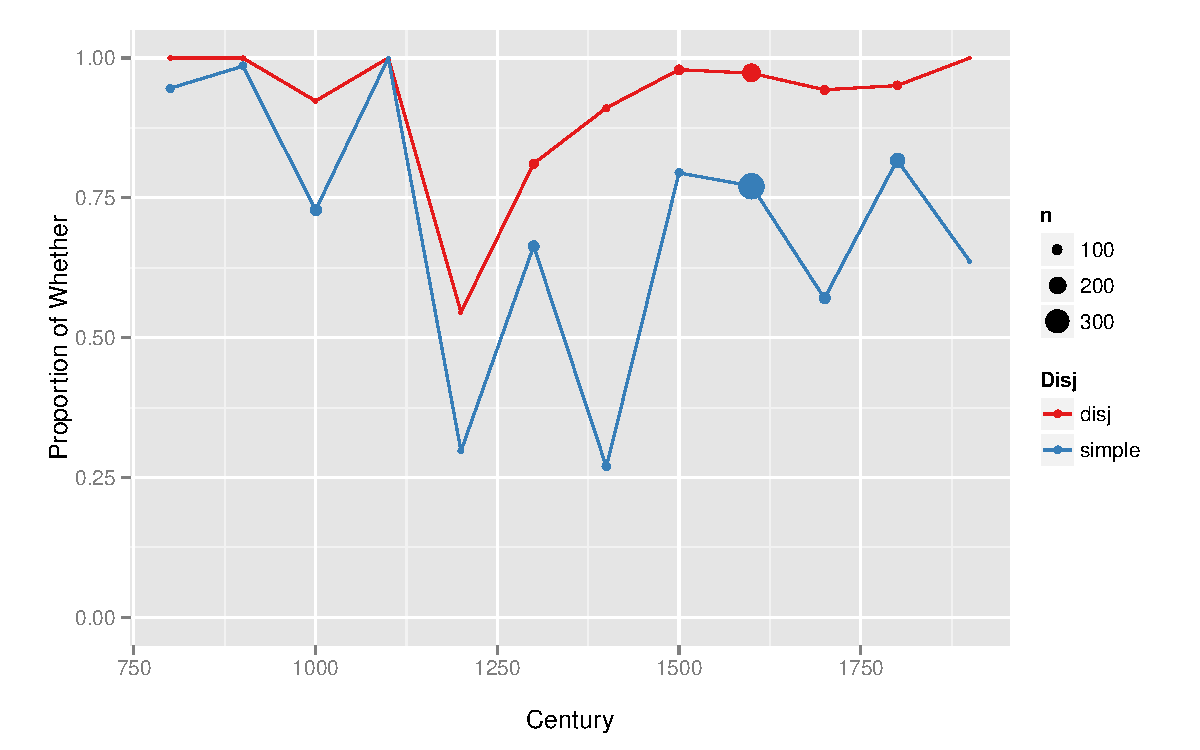
\includegraphics[width=1.1\textwidth]{whetherifEng.pdf}
%\end{textblock*}
%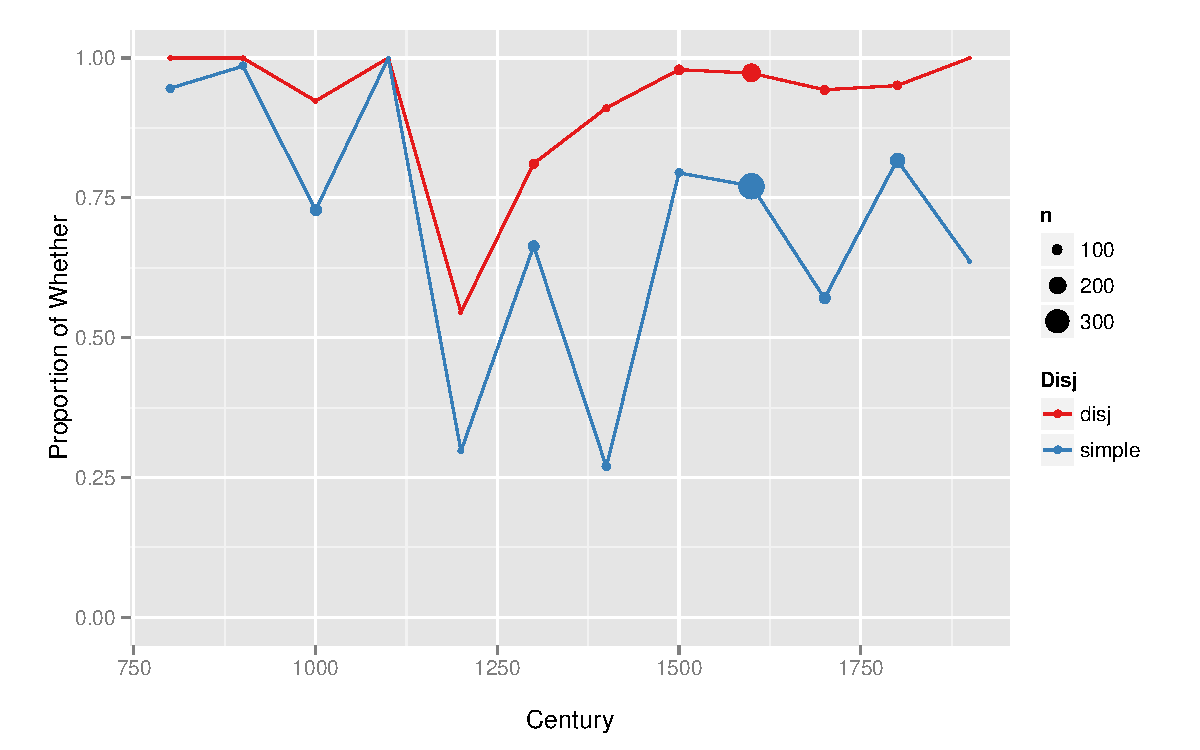
\includegraphics[scale = 0.5]{whetherifEng.pdf}
\end{center}
\end{frame}

%\begin{frame} 
% \frametitle{}
% \begin{center}
%                    
%\begin{tabular}{llllll}
%\hline
%  & Df & Deviance & Resid. Df & Resid. Dev &  Pr(>Chi) \\
%\hline
%NULL &   &    &            1928  &   1928.3 &  \\
%Disj   &    1 & 152.667  &    1927  &   1775.7 & < 2e-16\\
%Time     &    1  &  1.480  &    1926  &   1774.2  & 0.224\\
%Disj:Time  & 1  &  5.401   &   1925   &  1768.8 &    \textbf{0.0201}\\
%\hline
%\end{tabular}
%\end{center}
%\begin{itemize}
%\item A model without an interaction between Disjunction and Time fits significantly worse.
%\item Note that there is no clear effect of Time on \textsl{whether} use in general; the interesting effect is an interaction between Time, Disjunction, and  \textsl{whether} use.
%\item In other words, \textsl{whether} is not in decline, being replaced by \textsl{if}, but rather they are diverging from each other in use, specializing for the two contexts.
%\end{itemize}
%\end{frame}
%
%\begin{frame} 
% \frametitle{English, Logistic Model, N = 1929}
% \begin{center}
% \begin{textblock*}{125mm}(0mm,14mm)
%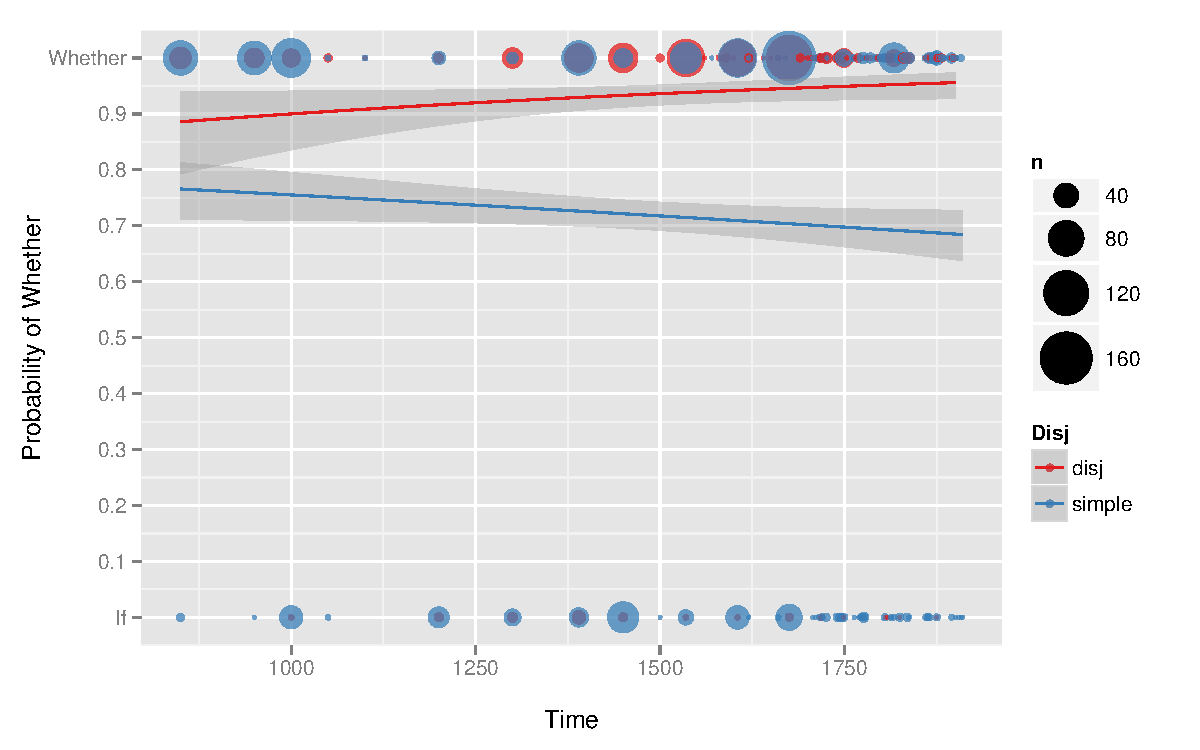
\includegraphics[width=109mm,height=80mm,clip=true,trim=0mm 0mm 0mm 0mm]{whetherifEngmodel.pdf}
%\end{textblock*}
% \end{center}
%\end{frame}
%
\begin{frame}{Replacement in Icelandic (N = 397 clauses)}

\begin{center}
IcePaHC \small{(Wallenberg, AK Ingason, EF Sigurðsson, \& E Rögnvaldsson 2011)}
% \begin{textblock*}{125mm}(0mm,14mm)
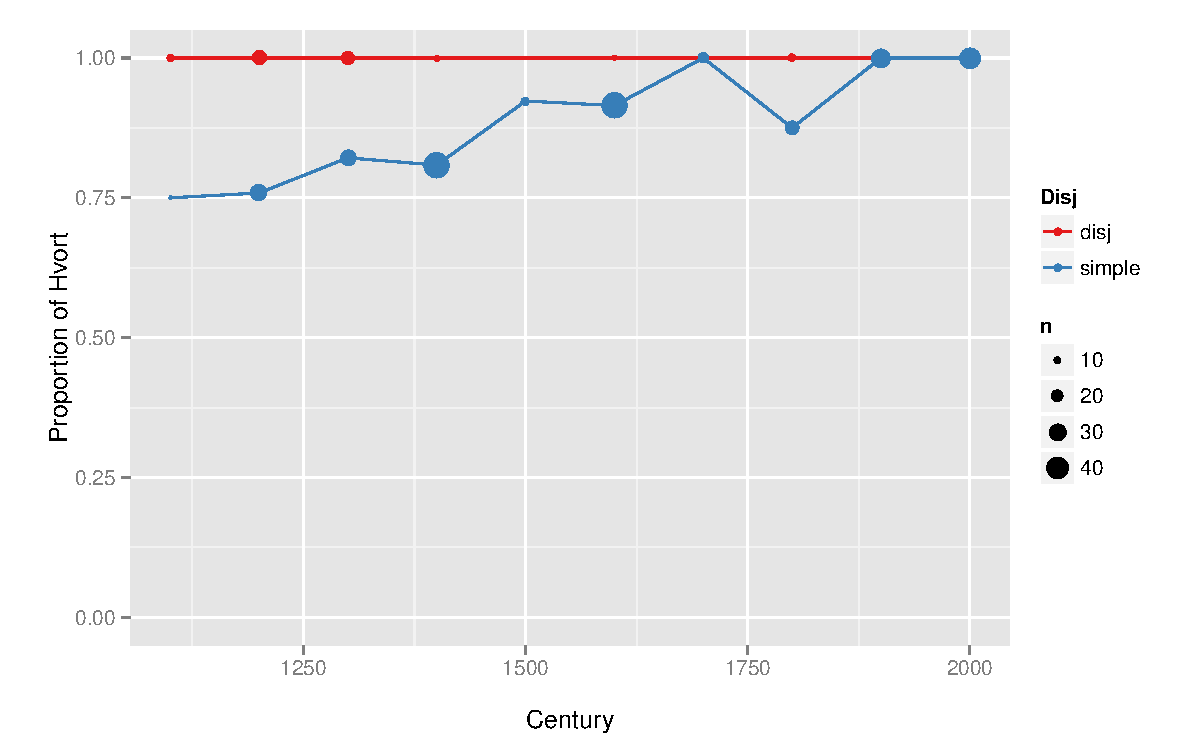
\includegraphics[width=1.1\textwidth]{whetherifIce.pdf}
%\end{textblock*}

\end{center}
\end{frame}

%\begin{frame} 
% \frametitle{Icelandic, Logistic Model, N = 397}
% \begin{center}
% \begin{textblock*}{125mm}(0mm,14mm)
%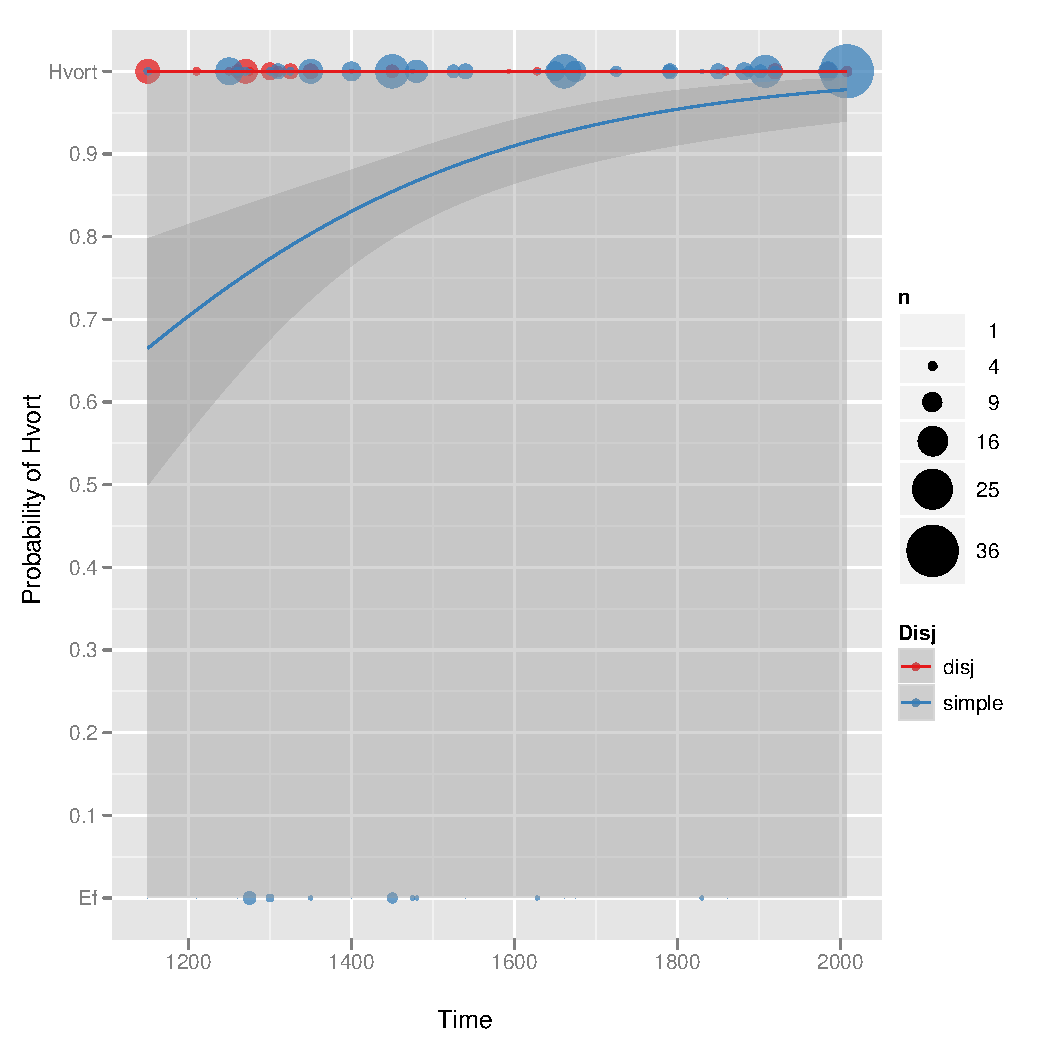
\includegraphics[width=109mm,height=80mm,clip=true,trim=0mm 0mm 0mm 0mm]{whetherifIcemodel.pdf}
%\end{textblock*}
% \end{center}
%\end{frame}
%
%
%\begin{frame}
%\frametitle{Whether/if Questions}
%
%\begin{exe}
%		\ex John wondered whether Mary was coming to the party.
%		\ex John wondered if Mary was coming to the party.
%\end{exe}
%\begin{itemize}
%	\item Is the frequency stable over time? Not in earlier English, but possibly in very recent history.	
%	\item Is it specialised for different speech styles (registers)? Yes, according to \citet{biberetal1999}.
%	\item Will they ever completely specialise for disjunction/simple? It depends on the strength of the style effect.
%\end{itemize}
%\end{frame}

%\section{Conclusions}
%\begin{frame}
%\frametitle{Conclusions}
%\begin{itemize}
%	\item We have shown that plausible reanalysis of \textsl{whether} in disjunctive contexts in Northwest Germanic led to its use in embedded \textsl{yes/no}-questions.
%	\item The effect of disjunctive contexts remains a crucial factor conditioning the choice between \textsl{if} and \textsl{whether} over the whole histories of English and Icelandic (in which it is categorical).
%	\item \textsl{whether} replaces \textsl{if} in Icelandic, but in English the two items specialise for different functions.
%	\item We suggested a reason for the difference between the two languages based on the continuing presence of the original reanalysis environment in Icelandic only (though this hypothesis would require more careful quantitative work to test).
%\end{itemize}
%\end{frame}
%
%\begin{frame}
%\frametitle{Conclusions and Future Research}
%\begin{itemize}
%	\item The data from the two languages illustrate the two possible outcomes for grammars that come into competition for use, according to the ``Blocking Effect''.
%	\item On the basis of this case study, we have suggested that the mechanism of competition for use could underlie all optional or variable syntactic phenomena, given:
%		\begin{itemize}
%			\item The Principle of Contrast as an acquisition strategy.
%			\item The mathematical nature of the dimension along which variants contrast (specialise).
%		\end{itemize}
%	\item Could we write a realistic, unified algorithm for acquisition, which predicts these effects? 
%\end{itemize}
%
%\end{frame}
%

\section{Stable Variation}
\begin{frame}
\frametitle{Stable Variation}
\textbf{Hypothesis:} Stable variation, i.e. optionality, results from categorical variants specializing along a continuous dimension.\\
\vspace{4mm}
There are many possible continuous dimensions, including language internal dimensions like
	\begin{itemize}
		\item weight (word length)
		\item prosodic accent (number of aligned prosodic peaks, degree of stress clash between two positions)
	\end{itemize}
and language external dimensions like
	\begin{itemize}
		\item style
		\item speech rate
	\end{itemize}
\end{frame}

\subsection{Example: Topicalization}
\begin{frame}
\frametitle{Example: English Topicalization}

\begin{itemize}
	\item Is the frequency stable over time? Probably, at least since Late Middle English \citep{speyer2010}.
	\item Is it specialized for different speech styles (registers)? Not that we know of.
	\item Is it sensitive to prosody? Definitely \citep{speyer2010}.
\end{itemize}

	\begin{exe}

	\ex  The first she'll feed mouse chow, the second she'll feed veggies, and \textbf{the third} she'll feed  \textbf{junk food}.\\

	\ex  ? The first Anders will feed, the second Joel will feed, and the third Wim will feed. \\

	\ex  ?? Joel Anders will pay, Jill Wim will pay, and Ann Maggie will pay. \\

	\end{exe}
\end{frame}

\subsection{Example: -\textipa{In}$\sim$-\textipa{IN}}
\begin{frame}{Example: -\textipa{In}$\sim$-\textipa{IN}}
	\begin{exe}
			\ex John has been \{singing/singin'\}.
			\ex \{Dunking/Dunkin'\} Donuts.
	\end{exe}
	\begin{itemize}
		\item Is the frequency stable over time? Probably, as the variation has its roots in OE morphology (Houston 1985), and both variants were present in Middle English texts \citep{labov1989}.
		\item Is it specialized for different grammatical contexts? Yes, in part, along a nominal$\leftrightarrow$verbal dimension \citep{labov1989}.
		\item It it specialized for different speech styles? Yes, in part, along a continuous dimension of formality.
	\end{itemize}


\end{frame}

\subsection{Acquisition Simulation}
\begin{frame}{Example: -\textipa{In}$\sim$-\textipa{IN}}
	A proof of concept simulation shows that plausibly, under minimal acquisition assumptions:
	\begin{itemize}
	\item Variants specialize along a continuous dimension like style.
	\item For a continuous dimension, the process will stabilize at \textbf{partial} specialization. 
	\item[ ] \begin{itemize}
		\item[\textbf{Gen 0:}]  -\textipa{In}$\sim$-\textipa{IN} doublet is innovated, with no stylistic conditioning. \textbf{Gen 0} picks a style to speak in, and produces a variant, repeats. 
		\item[\textbf{Gen 1:}]  \textbf{Gen 1} learns an estimate for the style value of -\textipa{In}, \textipa{IN}, as soon as she hears the first tokens of each from \textbf{Gen 0}. She adjusts this estimate as she gets more data from \textbf{Gen 0}.
		\item[\textbf{Gen 2:}] \textbf{Gen 1} picks a style, produces one of the variants with a probability weighted by how far her style estimates are from the current style, repeats. \textbf{Gen 2} learns style estimates for variants as above.
	\end{itemize}
	\end{itemize}
\end{frame}


%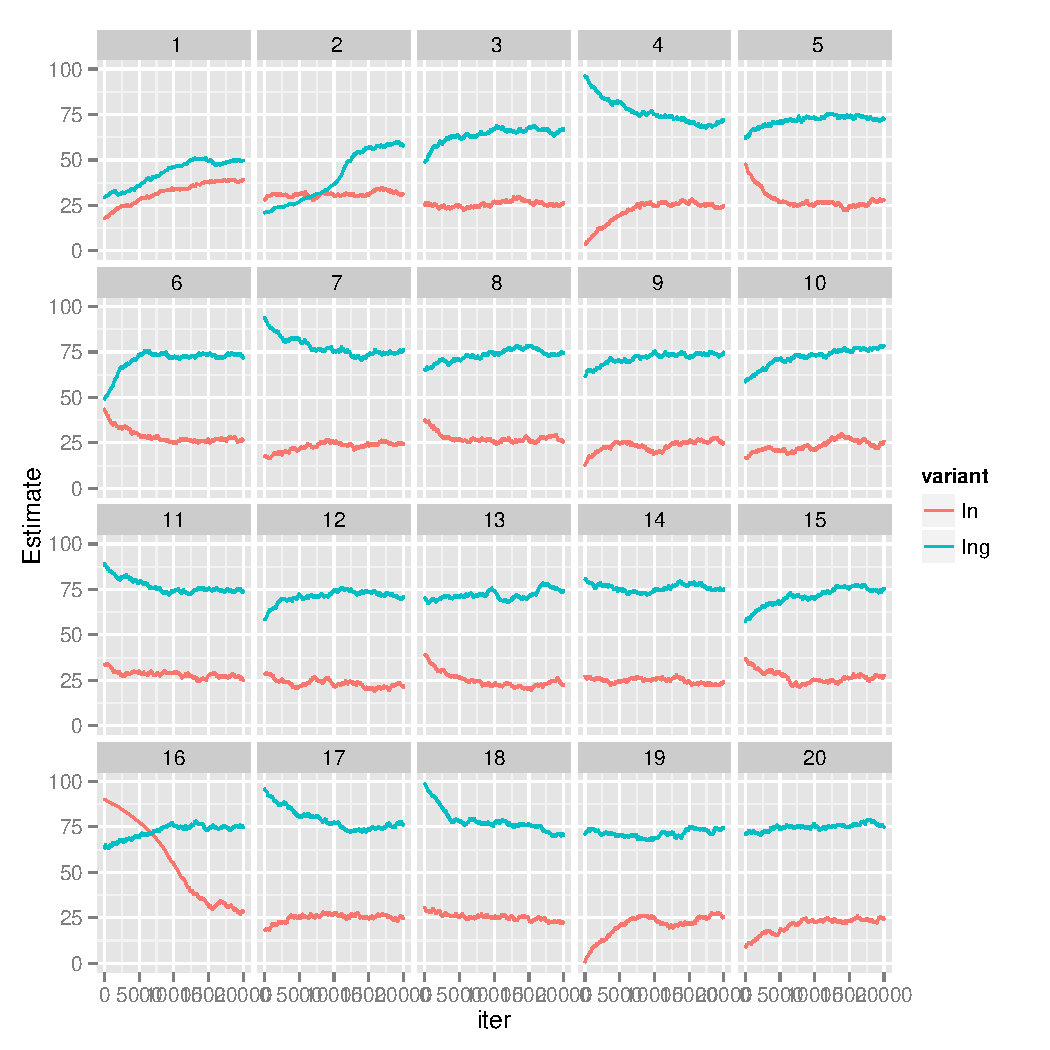
\includepdf{niceExample20000Run.pdf}





\section{Conclusions}
\begin{frame}{Conclusions}
	\begin{block}{Conclusions}
		\begin{itemize}
			\item Within syntax, only one formal account of optionality is available, the same one that accounts for language change: Competing Grammars.
			\item This results in replacement, specialization, or stable variation (true optionality).
			\item The latter is (only) the result of mapping categorical variation onto a continuous dimension of specialization.
			\item An acquisition simulation shows how stable variation can emerge under a minimal Principle of Contrast.
			\item It is possible and desirable to extend this formal account to other domains of variation, like morphology and phonology.
		\end{itemize}
	\end{block}


\end{frame}

\begin{frame}{Conclusions}
	\begin{block}{Further Work}
		\begin{itemize}
			\item Figure out what factors influence specialisation vs replacement, as they do not \textbf{appear} to be deterministic.
			\item Figure out how to appropriately parameterize phonological variation.
		\end{itemize}
	\end{block}

\end{frame}



\begin{frame}[allowframebreaks]
\frametitle{References}
\newcommand*{\newblock}{natbib}
\bibliographystyle{linquiry2}
\bibliography{joelrefs}
\end{frame}




\end{document}